\documentclass{article}
\usepackage{graphicx}
\usepackage[section]{placeins}
\makeatletter
\AtBeginDocument{%
  \expandafter\renewcommand\expandafter\subsection\expandafter{%
    \expandafter\@fb@secFB\subsection
  }%
}
\makeatother

\title{DUNE Flux Predicition Uncertainties for the DUNE Far Detector Technical Design Review Analysis}
\author{Luke Pickering}
\date{\today}

\begin{document}
\maketitle

\abstract{This Technical note describes an update of the DUNE flux  prediction prior uncertainties. It is meant to be read in the context of previous notes \cite{} and \cite{}. The two significant additions in this analysis are the inclusion of a range of near detector predictions off axis for use in DUNE-PRISM studies and the description of ready-to-use flux uncertainty tools based on an eigenvalue decomposition of the total flux matrix.}

\section{Flux Predictions}

All flux predictions in this document were produced using \texttt{g4lbne v3r5p4}, \texttt{GEANT 4.10.3p3}, and where applicable a slightly modified version of \texttt{PPFX vX}\footnote{No physics modifications were made so these results should be exactly reproducible}. The predictions were based upon the macro \texttt{OptimizedEngineeredNov17.mac}, which was modified where neccessary to move beamline components or alter running conditions.

The 'nominal' near detector (574 m) flux prediction for each horn polarity, neutrino species, and for 6 on- and off-axis positions can be see in Fig.\ref{fig:flux_predictions__on_axis}--\ref{fig:flux_predictions__off_axis}.

\begin{figure}
  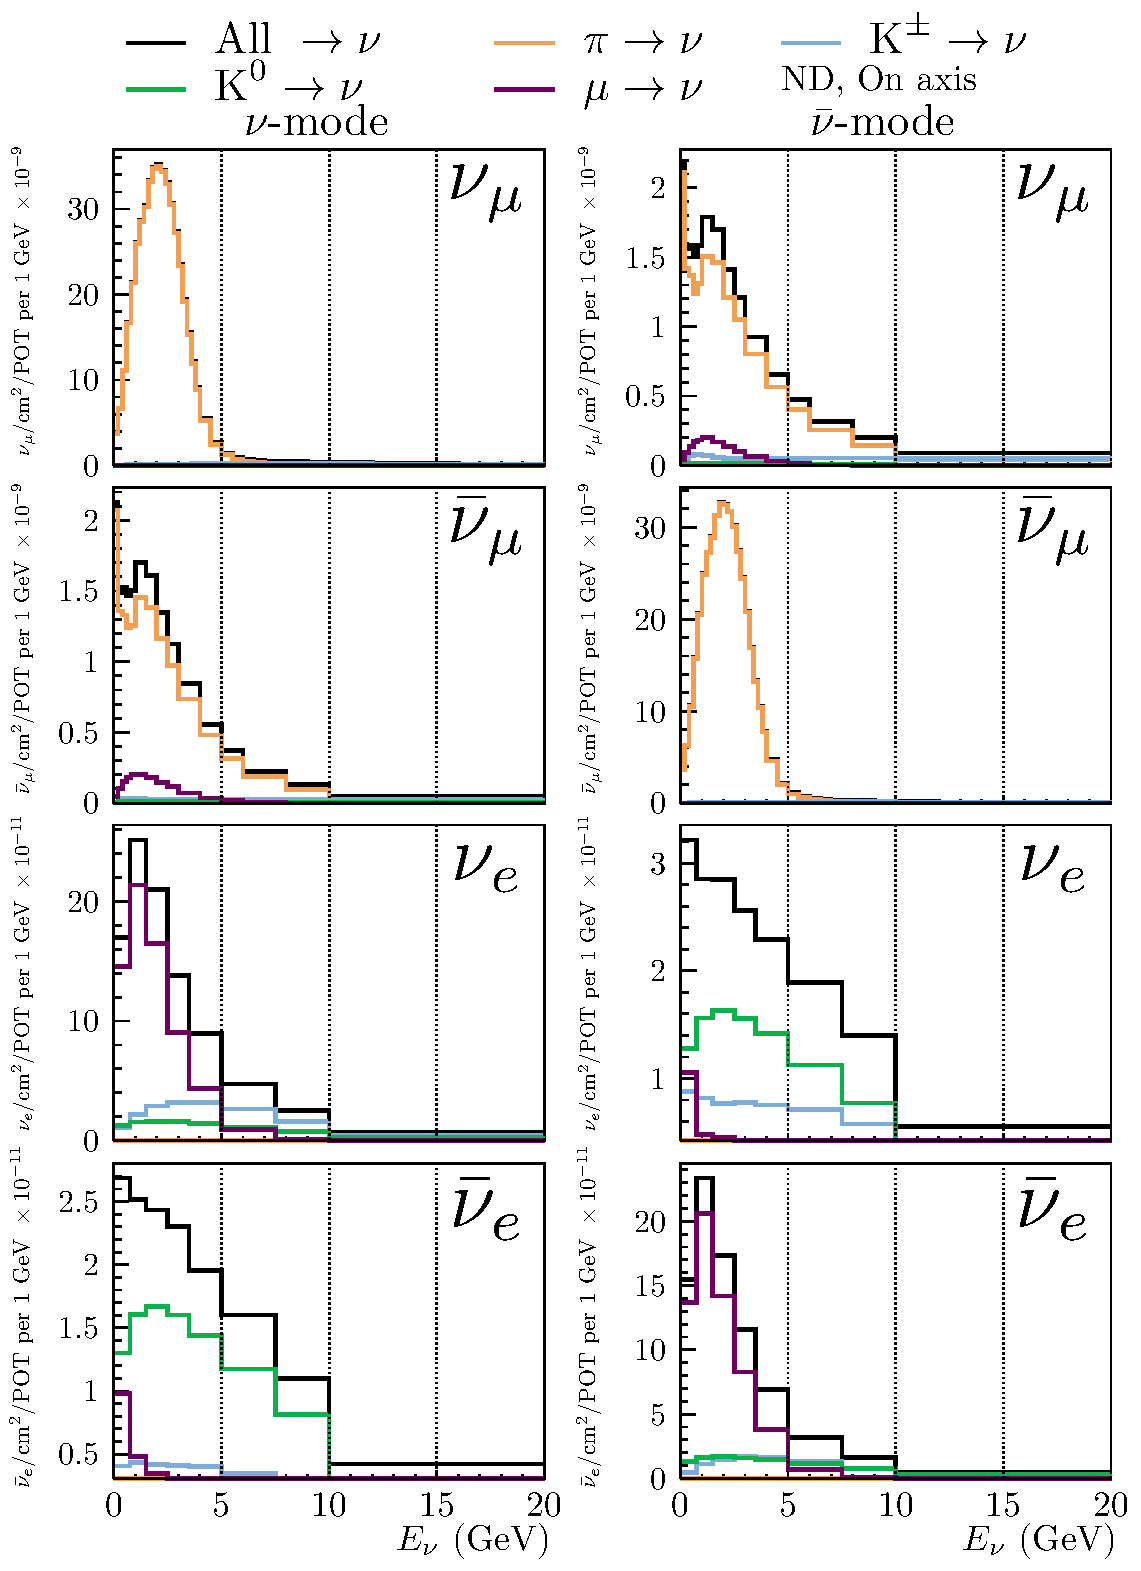
\includegraphics[width=\textwidth]{plots/fluxpredcompvar/ND_HadronParentFluxComponents_0m_offaxis}
  \caption{DUNE Flux prediction averaged over a $6\times 3\times 5\,\textrm{m}^{3}$ volume on axis at 574 m from the proton beam target station. The left hand set of figures shows the prediction when running with positive (negative) horn current (\textit{i.e.} mostly matter (anti-matter)). The prediction of each neutrino species in each horn current configuration is separated separated by the particle species that decayed to produce a given neutrino.}
  \label{fig:flux_predictions__on_axis}
\end{figure}
\begin{figure}
  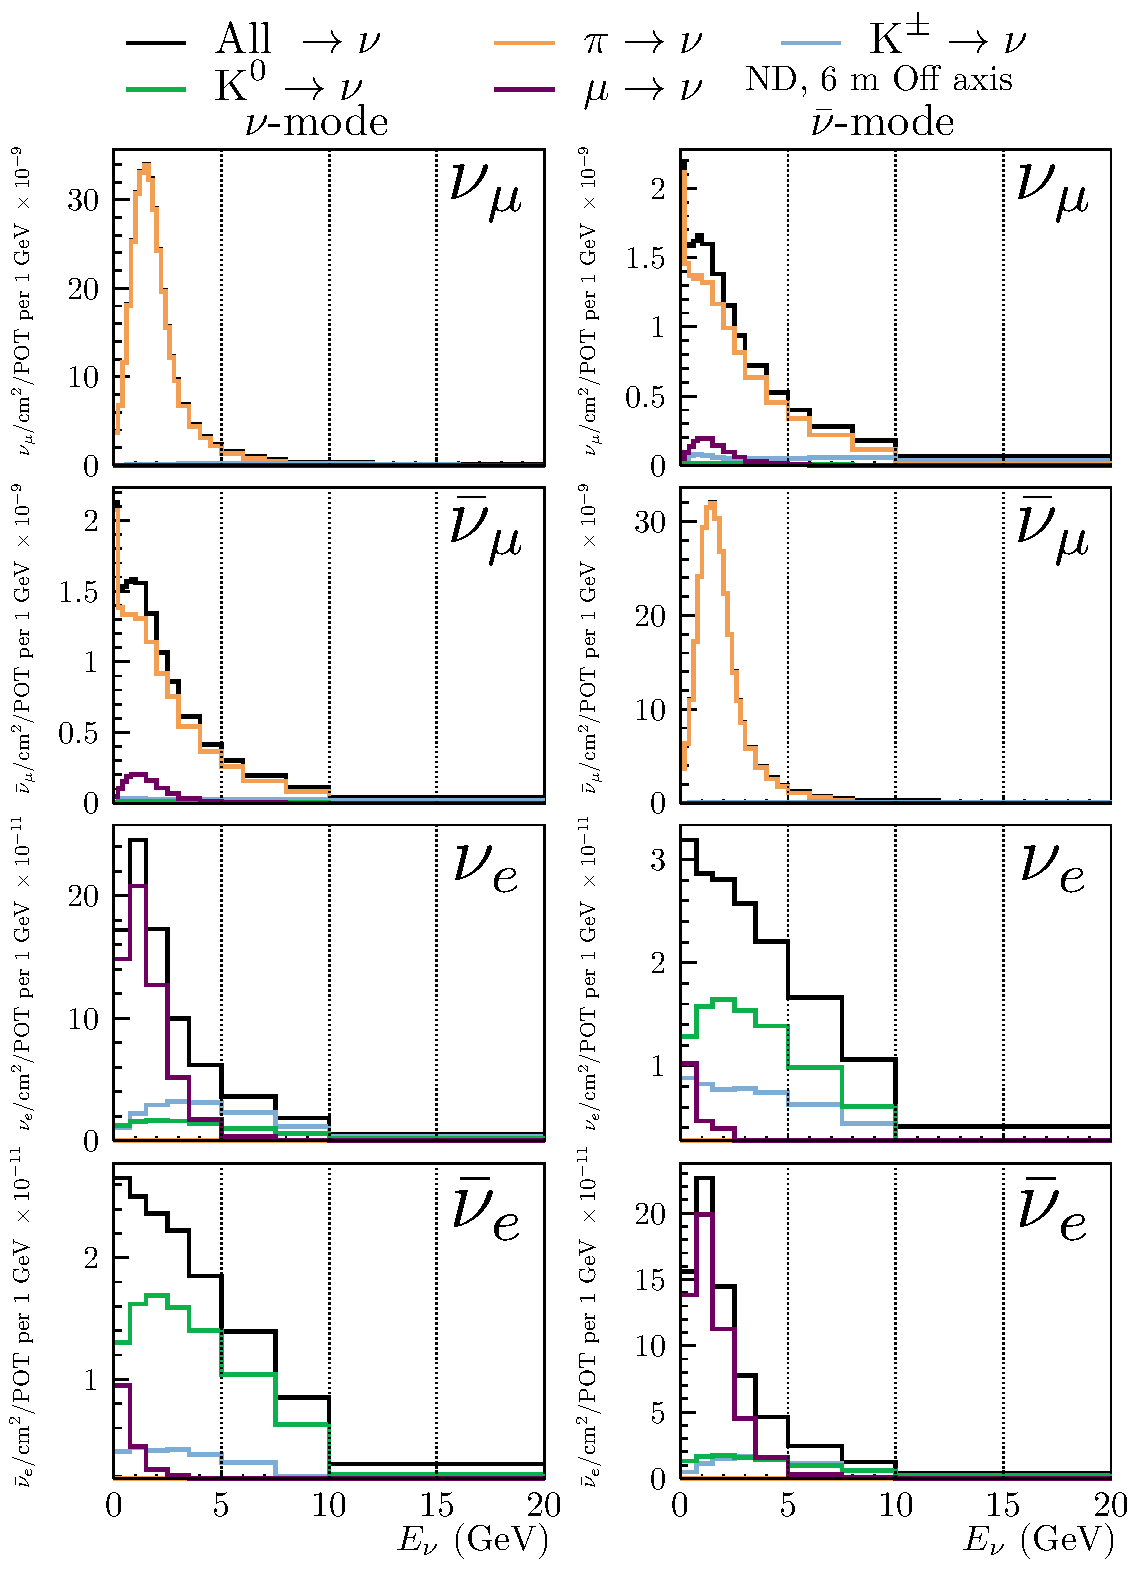
\includegraphics[width=\textwidth]{plots/fluxpredcompvar/ND_HadronParentFluxComponents_6m_offaxis}
  \caption{DUNE Flux prediction averaged over a $6\times 3\times 5\,\textrm{m}^{3}$ volume 6 m laterally off beam axis at 574 m from the proton beam target station. The left hand set of figures shows the prediction when running with positive (negative) horn current (\textit{i.e.} mostly matter (anti-matter)). The prediction of each neutrino species in each horn current configuration is separated separated by the particle species that decayed to produce a given neutrino.}
\end{figure}
\begin{figure}
  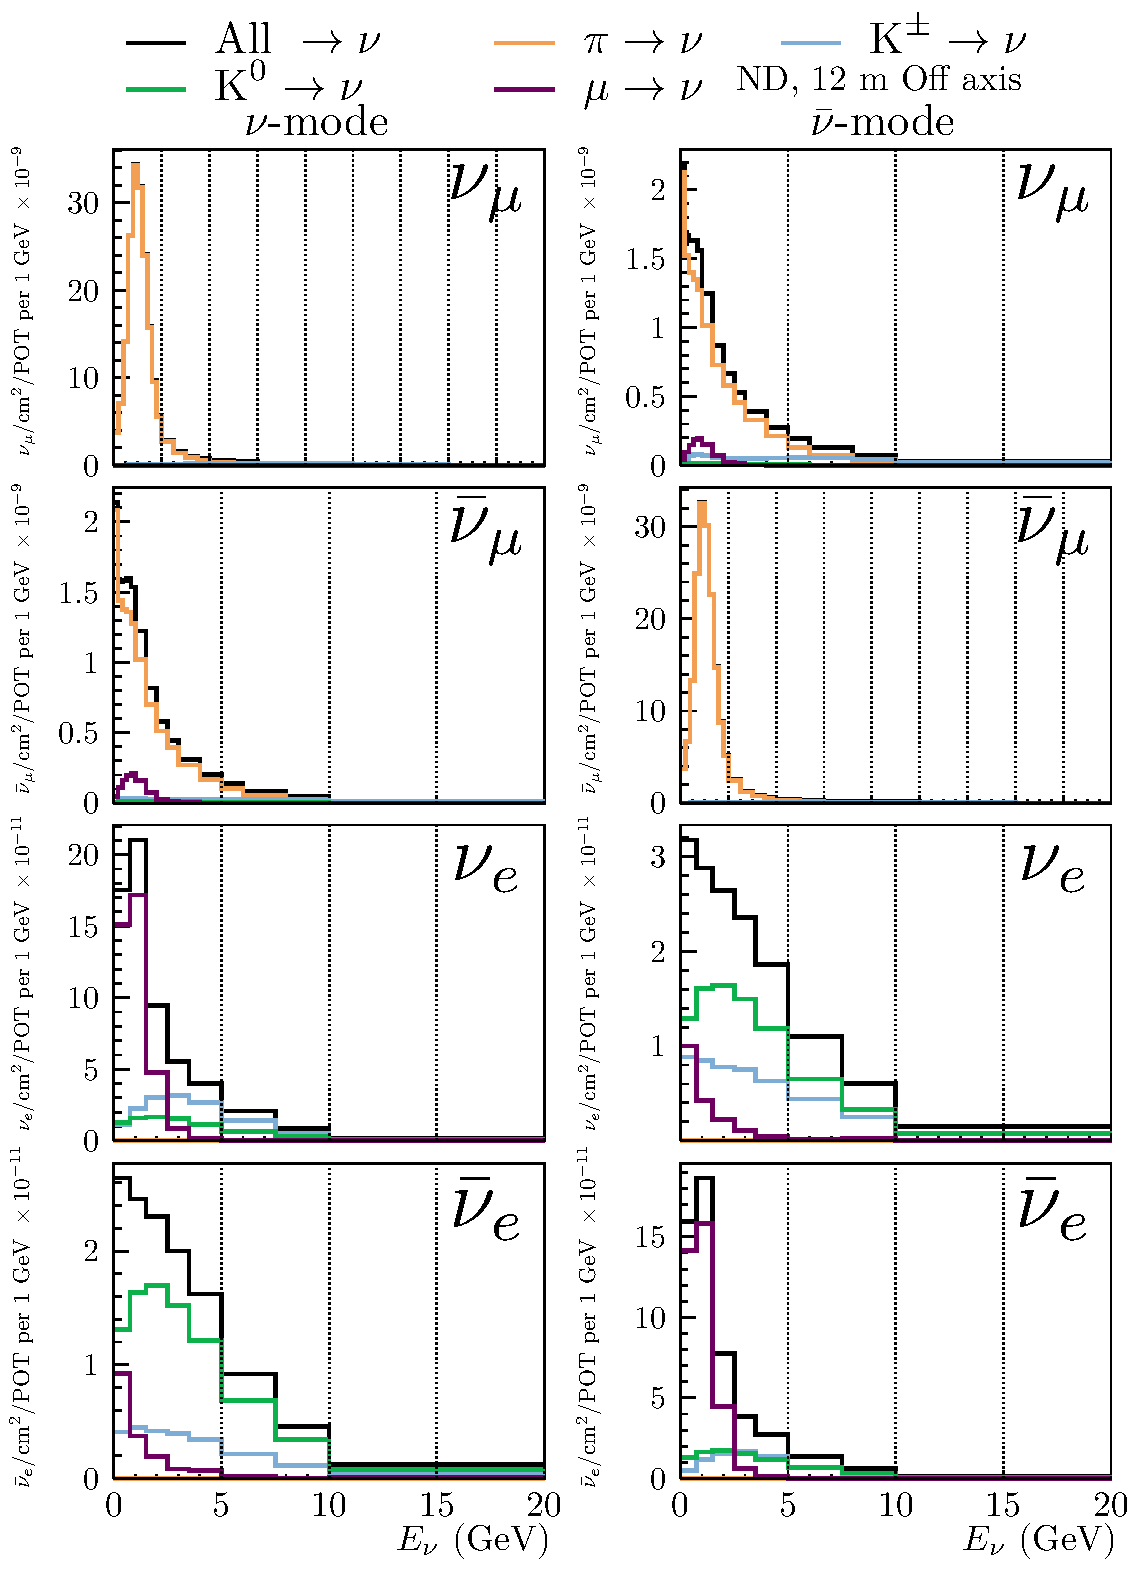
\includegraphics[width=\textwidth]{plots/fluxpredcompvar/ND_HadronParentFluxComponents_12m_offaxis}
  \caption{DUNE Flux prediction averaged over a $6\times 3\times 5\,\textrm{m}^{3}$ volume 12 m laterally off beam axis at 574 m from the proton beam target station. The left hand set of figures shows the prediction when running with positive (negative) horn current (\textit{i.e.} mostly matter (anti-matter)). The prediction of each neutrino species in each horn current configuration is separated separated by the particle species that decayed to produce a given neutrino.}
\end{figure}
\begin{figure}
  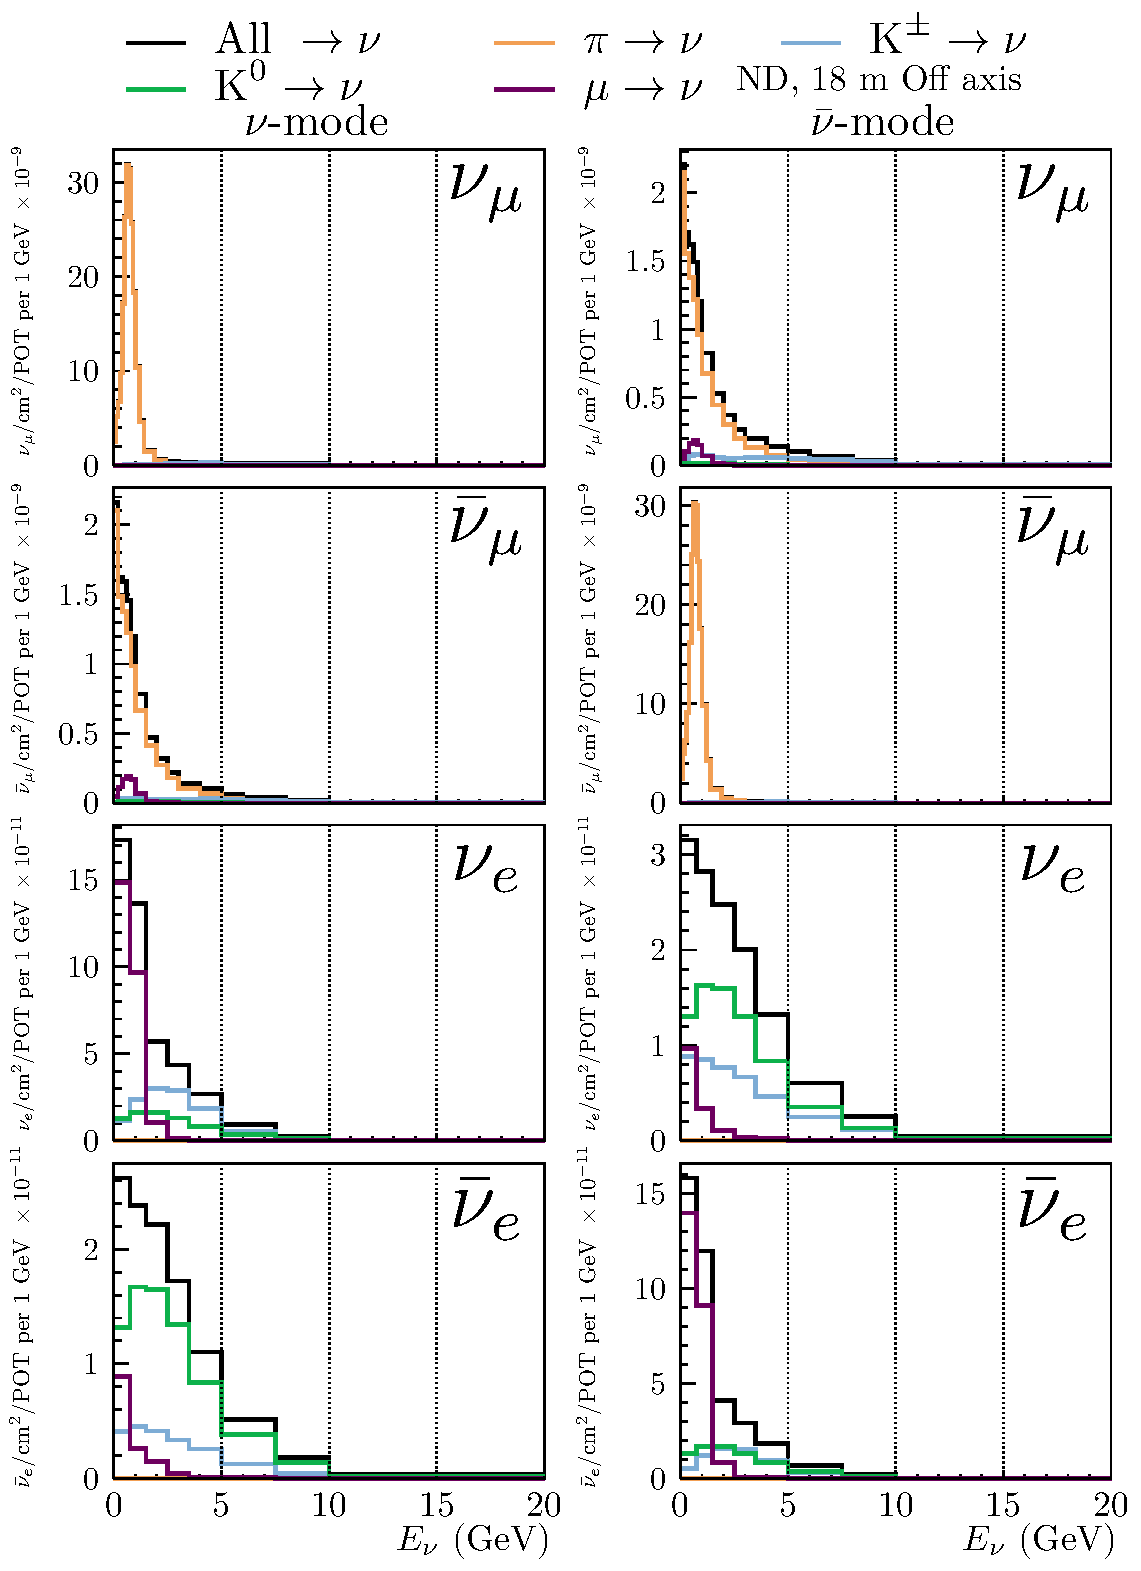
\includegraphics[width=\textwidth]{plots/fluxpredcompvar/ND_HadronParentFluxComponents_18m_offaxis}
  \caption{DUNE Flux prediction averaged over a $6\times 3\times 5\,\textrm{m}^{3}$ volume 18 m laterally off beam axis at 574 m from the proton beam target station. The left hand set of figures shows the prediction when running with positive (negative) horn current (\textit{i.e.} mostly matter (anti-matter)). The prediction of each neutrino species in each horn current configuration is separated separated by the particle species that decayed to produce a given neutrino.}
\end{figure}
\begin{figure}
  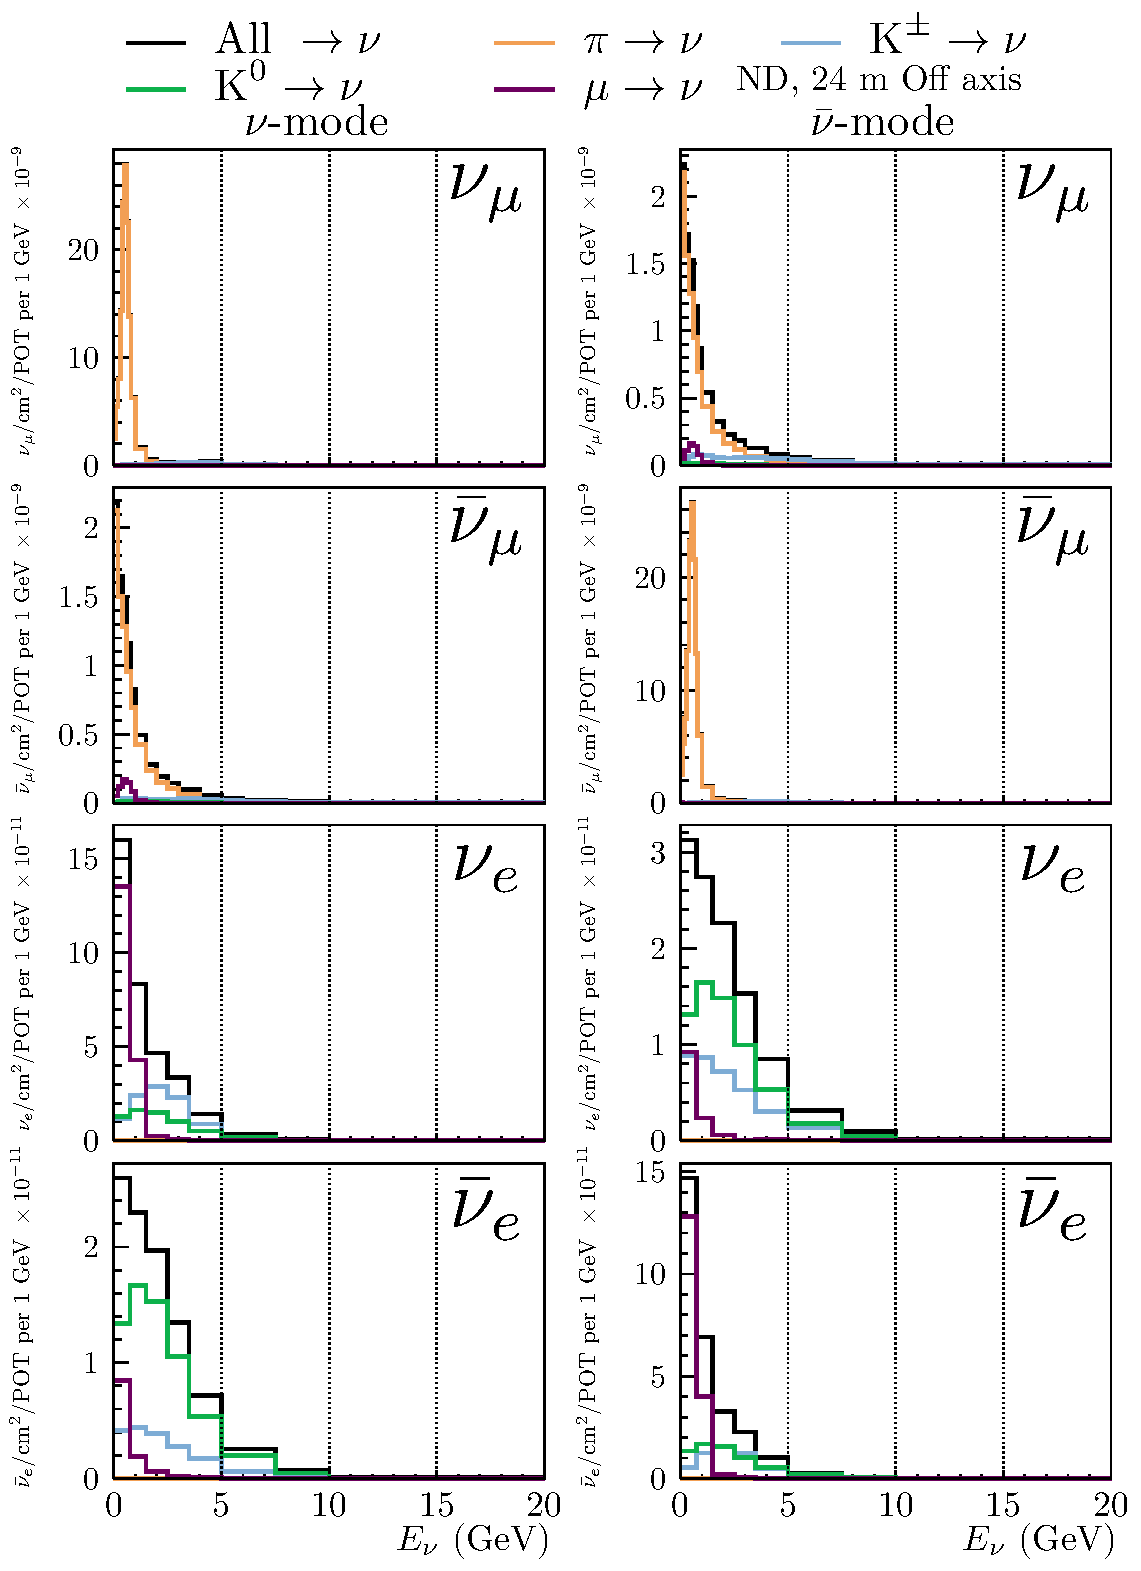
\includegraphics[width=\textwidth]{plots/fluxpredcompvar/ND_HadronParentFluxComponents_24m_offaxis}
  \caption{DUNE Flux prediction averaged over a $6\times 3\times 5\,\textrm{m}^{3}$ volume 24 m laterally off beam axis at 574 m from the proton beam target station. The left hand set of figures shows the prediction when running with positive (negative) horn current (\textit{i.e.} mostly matter (anti-matter)). The prediction of each neutrino species in each horn current configuration is separated separated by the particle species that decayed to produce a given neutrino.}
\end{figure}
\begin{figure}
  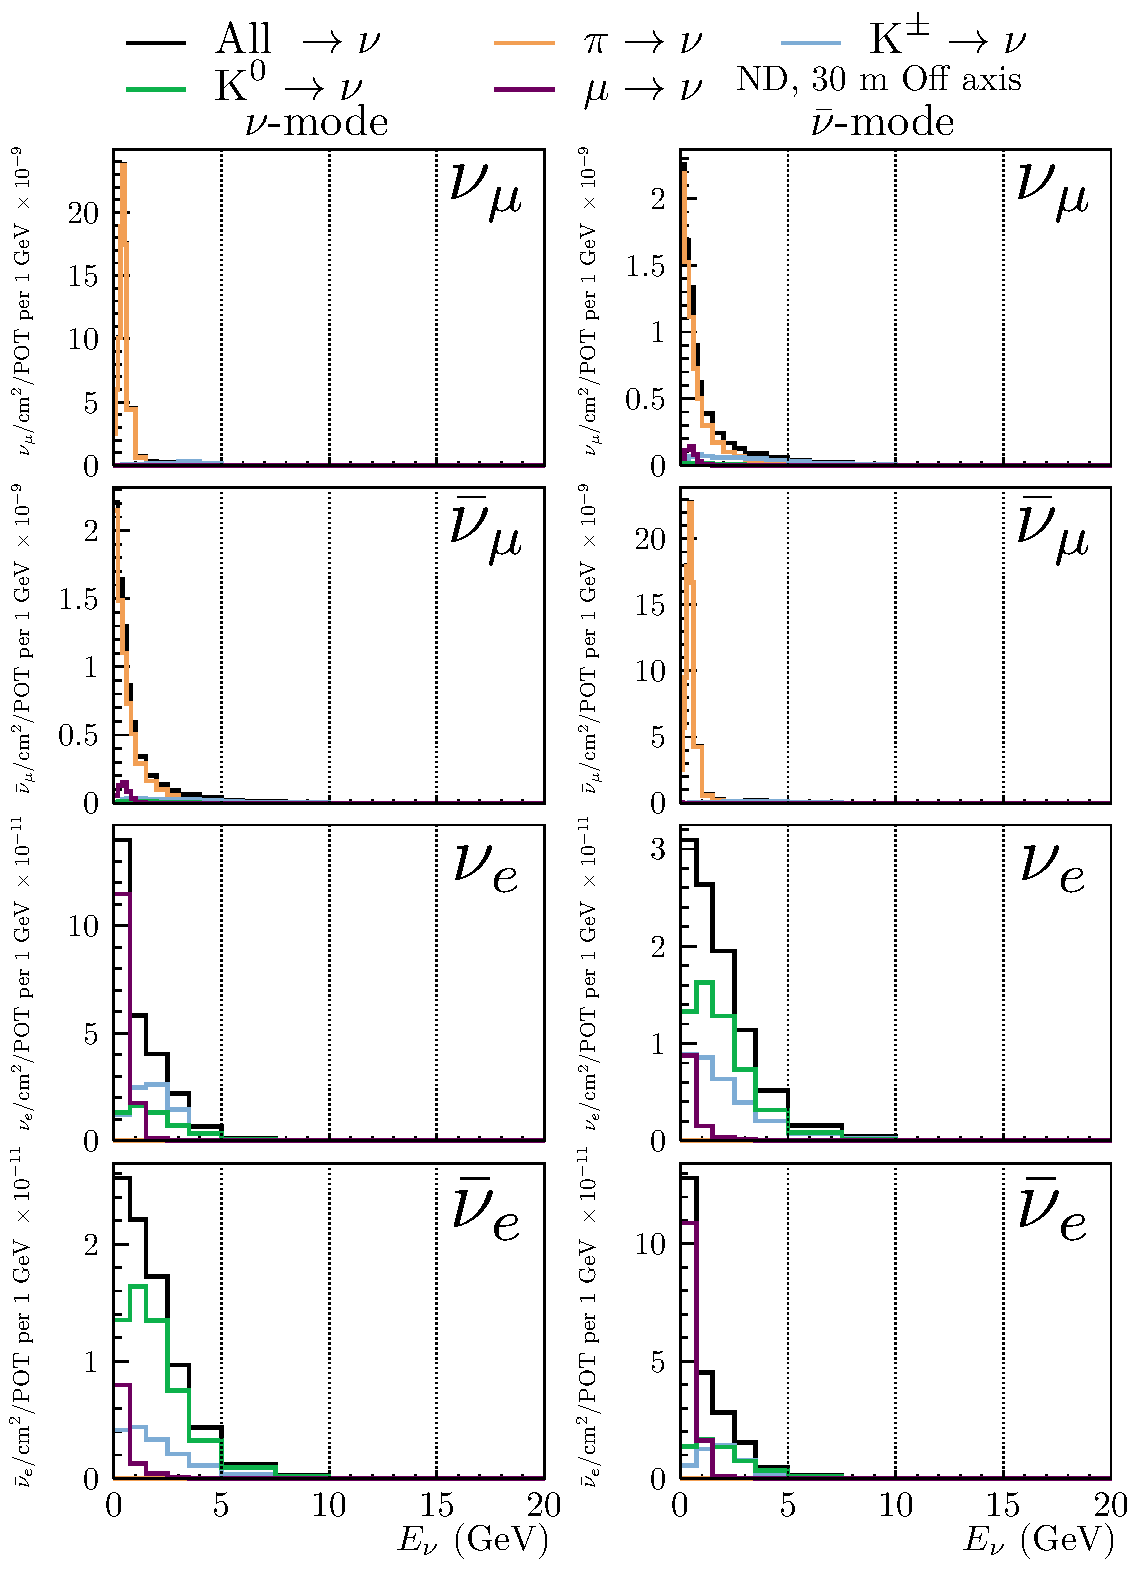
\includegraphics[width=\textwidth]{plots/fluxpredcompvar/ND_HadronParentFluxComponents_30m_offaxis}
  \caption{DUNE Flux prediction averaged over a $6\times 3\times 5\,\textrm{m}^{3}$ volume 30 m laterally off beam axis at 574 m from the proton beam target station. The left hand set of figures shows the prediction when running with positive (negative) horn current (\textit{i.e.} mostly matter (anti-matter)). The prediction of each neutrino species in each horn current configuration is separated separated by the particle species that decayed to produce a given neutrino.}
  \label{fig:flux_predictions__off_axis}
\end{figure}

\section{Methodology}

\subsection{Error determination}
\label{sec:methodology__error_determination}

The methodology for error propagation follows the previous notes closely.
There are 3 types of systematic variation used in this analysis: firstly, discrete variations where only a single shifted prediction is made and compared to the 'nominal' prediction to determine the magnitude of the effect. These could come from non-continuous variations, but practically in this analysis, all discrete shifts are continuous systematic variations of which only a single point is sampled. For such a variation the relevant component of the total error matrix is determined in the usual way by:
\[\mathbf{C} = \left(\vec{v}-\bar{n}\right)\left(\vec{v}-\bar{n}\right)^{\mathrm{T}}\label{eqn:covmx},\]
where $\vec{v}$ is the shifted prediction and $\bar{n}$ is the nominal prediction.

It is worth noting here that a prediction, $\vec{x}$, may contain any number of sub-predictions produced under the same beam conditions, \textit{i.e.} two horn polarities with 4 neutrino species for each of six near and and one far detector volumes is the standard prediction configuration used in this analysis. The error analysis does not care about any specifics of the binning as long the final error calculated for the $i$-th component of a prediction $\vec{\phi}$ can be correctly re-associated to the correct beam-mode, species, detector volume, and energy bin when diseminating the final uncertainties.

The second type of systematic variation is one where more than one sample along a single degree of freedom is made, and each must be included simultaneously in the error analysis. An example of this is the uncertainty on the vertical position of the second horn, for which one prediction at $+0.5 mm$ and one at $-0.5 mm$ was used. Here a polynomial is fit to the shifted predictions in each bin, this follows the treatment in \cite{}, but here the polynomial order is always the same as the number of varied samples (i.e. one less than the number of points to be fit). The fitted polynomial is then evaluated at $+1$ in each bin, producing a varied prediction, $\vec{v}$. Eqn~\ref{eqn:covmx} is again used to produce the error matrix component from an uncertainty of this type.

The final type is one where a larger number of samples are taken from a higher dimensional space of nuisance parameters. The canonical and only uncertainties treated this way are the hadron production uncertainties. The underlying parameters are binned cross-section normalizations for a large number of interactions that GEANT can simulate during the proton and daughter particle propagation through the target and horn geometry. There are far too many parameters to treat individually like the focussing and alignment errors. Instead flux predictions for some number of random\footnote{These random throws are constrainted by (possibly correlated) priors informed by hadron production experiments. See \texttt{PPFX} notes\cite{} for more details.} throws within this ($\mathcal{O}\left(700\right)$ dimension) parameter space are calculated and used to asses the correlated uncertainties from hadron production errors. The component matrix is then formed by the generalization of Eqn~\ref{eqn:covmx} to $N$ samples:
\[\mathbf{C} = 1/N\sum^{i=0}_{i<N} \left(\vec{v_{i}}-\bar{n}\right)\left(\vec{v_{i}}-\bar{n}\right)^{\mathrm{T}}\label{eqn:covmxN}.\]

\subsection{Binning}

As a primary driver for this re-analysis was the inclusion of an error analysis for off axis positions at the near detector site, the energy binning needs to be treated somewhat carefully. This is for two main reasons, firstly, if the energy or off axis binnings are too fine, then the number of bins becomes large and standard analysis techniques to use flux constraints become impractical (matrix inversion and decomposition). Secondly, at further off axis positions, the flux peaks at a much lower energy than on axis ($0.6$ GeV vs. $\sim 2.3$ GeV), this means that if an error analysis is performed with a uniform energy binning as a function of off axis angle, then MC statistical noise at far off axis positions and higher energies can dominate and produce problematic results.

As a result, the analysis was performed using a custom histogram class, \texttt{TH2Jagged}, which subclasses the \texttt{TH2} from \texttt{ROOT}. It allows for 2D rectangular histogram with one axis defined as a function of the other axis. In this case, the energy binning is a function of the off-axis angle binning. As using custom classes is somewhat fiddly, the final output will not rely on the analyzer having access to this class. There are three binnings used in this analysis: one for the 'right sign' muon neutrino ($\nu_{\mu}$ in $\nu$-mode and $\bar{\nu}_{\mu}$ in $\bar{\nu}$-mode) , one for the 'wrong sign' muon neutrino ($\bar{\nu}_{\mu}$ in $\nu$-mode and $\nu_{\mu}$ in $\bar{\nu}$-mode), and a third for all electron-type neutrinos (which constitute $\sim 1\% $ of the total flux in any configuration). The binning definitions can be seen in Figs.

%Binning definitions

\section{Uncertainties Used}
\label{sec:uncertainties_used}
Table~\ref{tbl:uncertdefn} contains the systematic variations used. The 'type' of each variation as defined in \S~\ref{sec:methodology__error_determination} can be determined by the number of listed variations. Note that each of these sources of error are treated as independent. The \texttt{g4lbne} macro files used for each systematically varied prediction should be distributed with this note, the 'Name' column corresponds to the macro file used with the exception of the 'PPFX' variations which are calculated by reweighting the nominal prediction.

\begin{table}
\centering
\begin{tabular}{l|l|l}
Name & Category & Variations \\
\hline
PPFX & Hadron production & 100 throws about \texttt{PPFX} CV tune \\
\hline
DecayPipeRadius & Focussing & +10 cm \\
WaterLayer & Focussing & +0.5 mm \\
HornCurrent & Focussing & +3, -3 kA \\
TargetDensity & Focussing & +1.8, -1.8 \% \\
\hline
Horn1XShift & Horn Alignment & +3,+0.5, -0.5, -3 mm\\
Horn2XShift & Horn Alignment & +0.5, -0.5 mm \\
Horn1YShift & Horn Alignment & +0.5, -0.5 mm \\
Horn2YShift & Horn Alignment & +0.5, -0.5 mm \\
\hline
BeamTheta & Beam Alignment & 0.07 mrad tilt \\
BeamThetaPhi & Beam Alignment & 0.07 mrad tilt and $90^{\circ}$ rotation about $\hat{z}$ \\
BeamSigma & Beam Alignment & +0.1, -0.1 mm \\
BeamOffsetX & Beam Alignment & +0.45, -0.45 mm \\
\end{tabular}
\caption{The systematic variations used in this analysis.}
\label{tbl:uncertdefn}
\end{table}

\section{Results}

The following subsections present the bin-by-bin fractional uncertainties for each beam mode and neutrino species for the near on axis, near off axis, and far detector flux volumes. For each the error on the ratio of the near on axis and far detector prediction is also shown, as oscillation analyses generally make use of systematic cancellation between the near and far detector.

It should be noted that all plots shown in this section were produced using the eigenvalue decompositions of the relevant component error matricies, \textit{i.e.} the tools presented in \S~\ref{sec:analyzer_usage} were exercised to do this analysis.

\subsection{Hadron production}
\subsection{Focussing}
\subsection{Horn Alignment}
\subsection{Beam Alignment}
\subsection{Grouped}

\subsection{Analyzer Usage}
\label{sec:analyzer_usage}

The error matrix constructed from the variations described in \S~\ref{sec:uncertainties_used} can be incorporated into analyses in a number of ways. There are two common ways. Firstly, each beam mode, species, energy bin in which the uncertainties are calculate introduces a nuisance parameter to the analysis. The value of these nuisance parameters control the relative probability (weight) for events produced by true neutrinos that fall within the corresponding bin. The matrix can then be used to form a penalty term like,
\[\textrm{pen}(\left(\textbf{p}\right)=\textbf{p}\mathbf{C}^{-1}\textbf{p}^\mathrm{T},\]
where, $\textbf{p}$ is the vector of nuisance parameter values and $\mathbf{C}$, is the total error matrix. The nature of beamline uncertainties results in constraints that are often strongly correlated across beam modes, neutrino species, and energy bins. As a result, this method can prove problematic for gradient descent minimization. This method neccessarily introduces one parameter per beam mode, neutrino species, and energy bin, this number cannot be reduced without losing granularity. For finely binned uncertainties as a function of off axis angle, this number can be prohibitively large, $\mathcal{O}\left(1000)$.

The second method is conceptually similar but mechanically slightly more involved and can be used to elide the two problems highlighted for the first method. The total number of varied predictions that went into the analysis was presented here was 122, however, for even on-axis-only and coarse energy binning the number of columns and rows in $\mathbf{C}$ is likely to be $\mathcal{O}\left(200)$. The matrix $\mathbf{C}$ can be diagonalized and then only the most important $n$ eigenvectors and values used in error propagation---where $n<122$, as the eigenvectors corresponding to smaller eigenvalues will neccessarily be composed of just MC statistical noise. This decomposition can be conceptually thought of as a rotation from the basis of beam mode, neutrino species, and energy to an effective basis that captures the correlated constraint described by $\mathbf{C}$ across all simultaneously.

% Eigenvalues
% Top X Eigenvectors

\section{Terms}

\begin{itemize}
\item Nominal:
\item $\nu$-mode, positive horn current, and mostly matter beam are used interchangeably, with the first being the preferred form.
\item $\bar{\nu}$-mode, negative horn current, mostly anti-matter beam are used interchangeably, with the first being the preferred form.
\end{itemize}


\end{document}
